\section{Wild Data Redux}

In an earlier lecture, we worked with wild data for the first time by using the public Peloton API to look at the JSON file associated with a single workout. Now, we'll revisit that and go a bit further using our expanded toolkit. 


Here are some new topics we'll learn about along the way. 

\begin{enumerate}
    \item Missing data and interpolation 
    \item Binning numerical data
    \item \code{Categorical} data type
\end{enumerate}


First, we'll replicate the output graph shown below in the Peloton workout details. % and go a step past the details provided by Peloton to calculate the Normalized Power for this workout. \link{https://www.trainingpeaks.com/blog/what-is-normalized-power/}{Normalized Power} is a score used by cyclists to calculate the physiological cost of a workout. In the end, it'll just be a function we import and apply to a Series. 

\begin{center}
    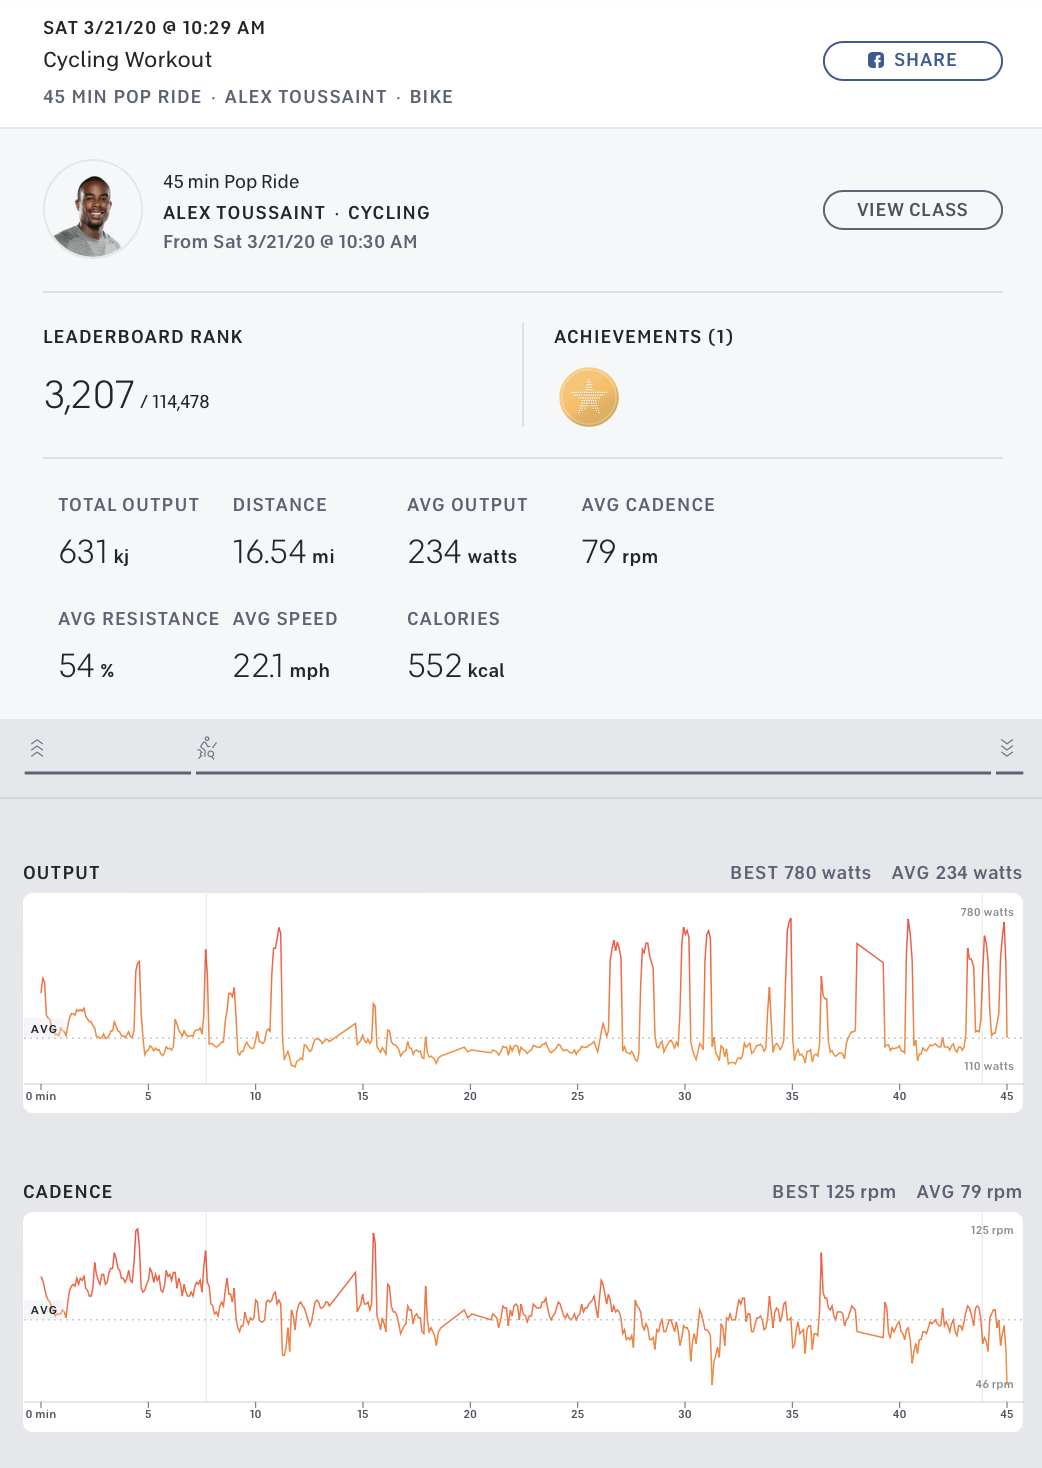
\includegraphics[width = 0.4\textwidth]{images/interpolated_workout_details.png}
\end{center}

Anyone can access data from a public Peloton profile, provided they have a login. Still, we'll bypass that step in these notes and suppose we already have the JSON files. 

\begin{lstlisting}
with open('redux_workout.json') as json_file:
    packets = json.load(json_file)
\end{lstlisting}

Check the keys with \code{.keys()} and you'll see we're interested in \code{packets['metrics']}. Further, this is a list, and we find the details for output at index level zero. 

\begin{lstlisting}
plt.subplots(figsize = (16,5))
plt.plot(pack2['metrics'][0]['values'])
plt.title("Workout Output")
plt.ylabel("Output (Watts)")
plt.savefig("redux_output1.pdf")
\end{lstlisting}

\begin{center}
    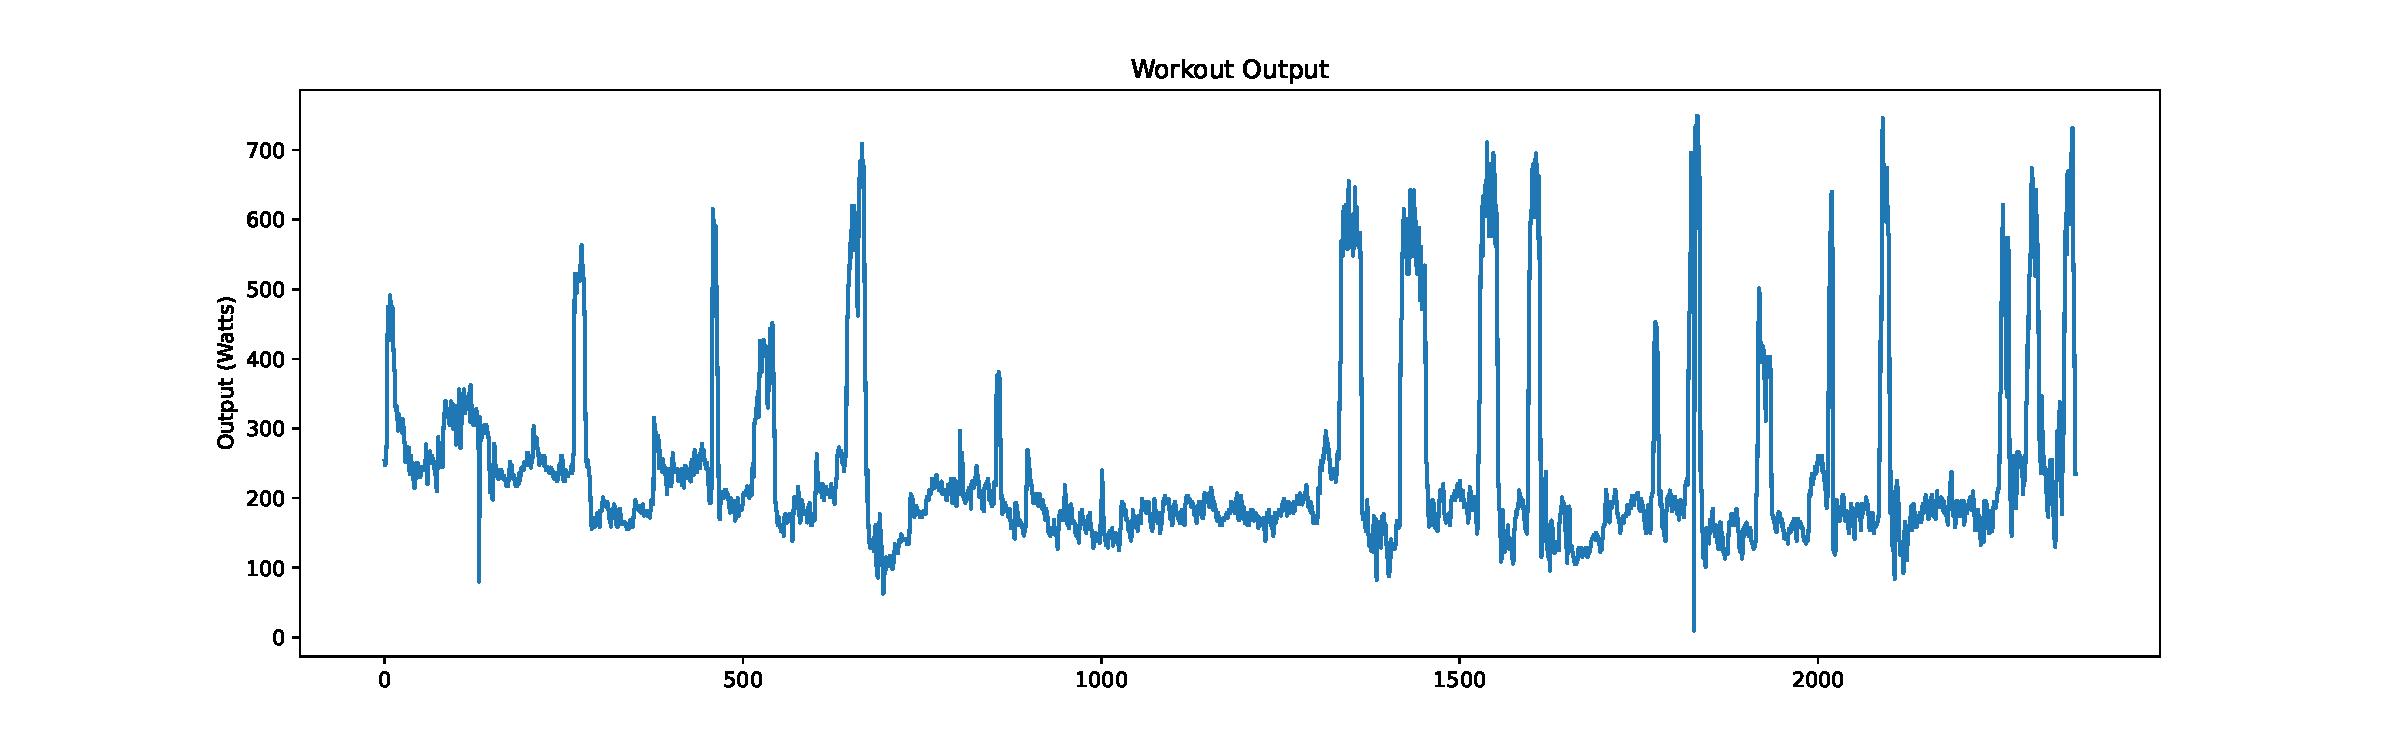
\includegraphics[width = .9\textwidth]{images/redux_output1.pdf}
\end{center}

We should see that this does \emph{not} match the workout details. For example, there is a straight line seen in the official details beginning at the 38 minute mark that does not show up in our plot. That's because there is missing data. We can verify this by checking the length of the packet array is not equal to the workout duration. 

With more inspection, you will find \code{packets['seconds_since_pedaling_start']}, which is itself a list of seconds. These can be interpreted as the corresponding workout times for each of the metric values (this is more Peloton knowledge or educated guessing than something immediately obvious from the data). These are the seconds for which the metrics were successfully captured. 
\begin{lstlisting}
plt.subplots(figsize = (16,5))
plt.plot(packets['seconds_since_pedaling_start'], packets['metrics'][0]['values'],
        color = 'black')
plt.title("Workout Output")
plt.ylabel("Output (Watts)")
plt.savefig("redux_output2.pdf")
\end{lstlisting}

\begin{center}
    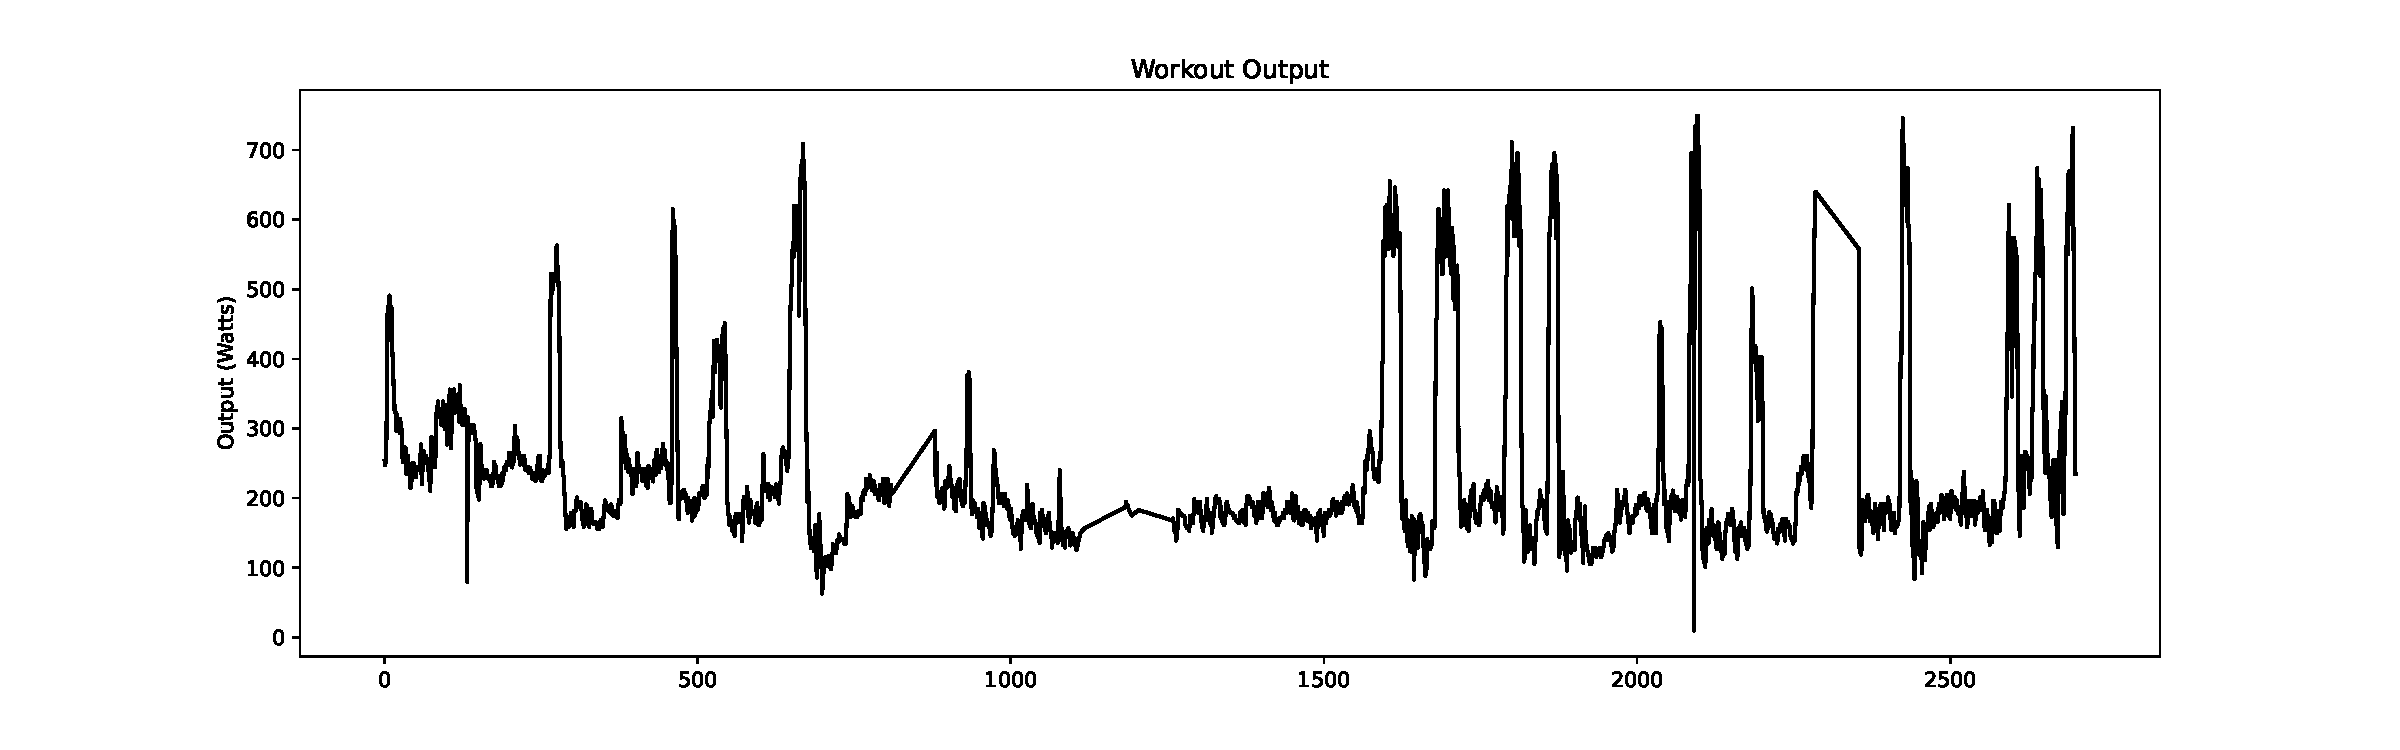
\includegraphics[width = .9\textwidth]{images/redux_output2.pdf}
\end{center}

Now, this matches the Peloton workout details (even if it's not as pretty). 

\subsection{Missing Data}

Above, we essentially interpolated the data linearly in the plot. That's because we drew a line between each value. So interpolation is done in a graph basically for free. In your data, you'll have to do more. The simplest way is to use the Series method \link{https://pandas.pydata.org/docs/reference/api/pandas.DataFrame.interpolate.html}{\code{interpolate()}}. This takes a Series with missing values and fills in those missing values


\begin{lstlisting}
interp_methods = ['linear', 'pad', 'zero', 'nearest', 'quadratic']

fig, ax = plt.subplots(len(interp_methods), 1, figsize = (10,7))
for key, s in enumerate(interp_methods):
    df['output'].interpolate(s).plot(ax = ax[key])
    ax[key].set_title(s)
plt.tight_layout()
plt.savefig("sample_interpolations.pdf")
\end{lstlisting}


\begin{center}
    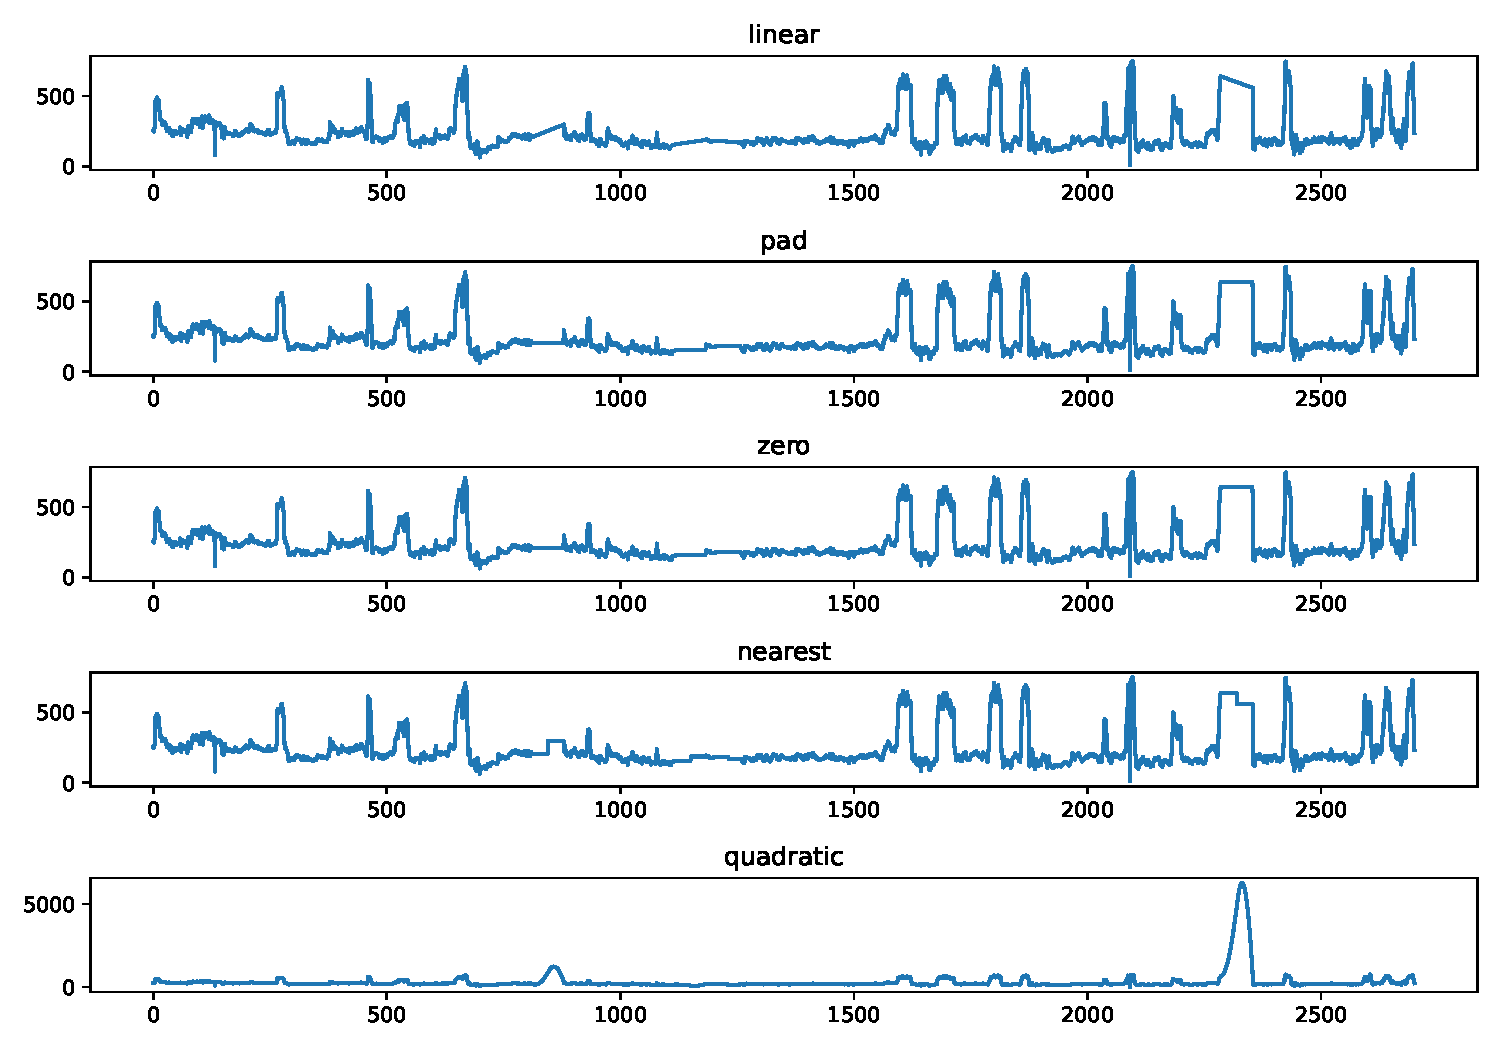
\includegraphics[width = .9\textwidth]{images/sample_interpolations.pdf}
\end{center}

\noindent Notice the very different $y$-axis limits for the quadratic interpolation. 

There are additional capabilities to use splines and more advanced ways of filling in the missing data. We won't cover that. Another low tech route is to use the \code{fillna()} Series method and related methods like \code{bfill()} and \code{ffill()}.


\begin{lstlisting}
fig, ax = plt.subplots(3, 1, figsize = (10,5))

# I include linear interpolation in orange/C1 for reference
df['output'].interpolate().plot(ax = ax[0], color = 'C1')
df['output'].bfill().plot(ax = ax[0], color = 'C0')
ax[0].set_title("Back Fill")

df['output'].interpolate().plot(ax = ax[1], color = 'C1')
df['output'].ffill().plot(ax = ax[1], color = 'C0')
ax[1].set_title("Forward Fill")


mean_output = df.output.mean()
df['output'].fillna(mean_output).plot(ax = ax[2])
ax[2].set_title("Mean")

plt.tight_layout()
plt.savefig("fillna_examples.pdf")
\end{lstlisting}

\begin{center}
    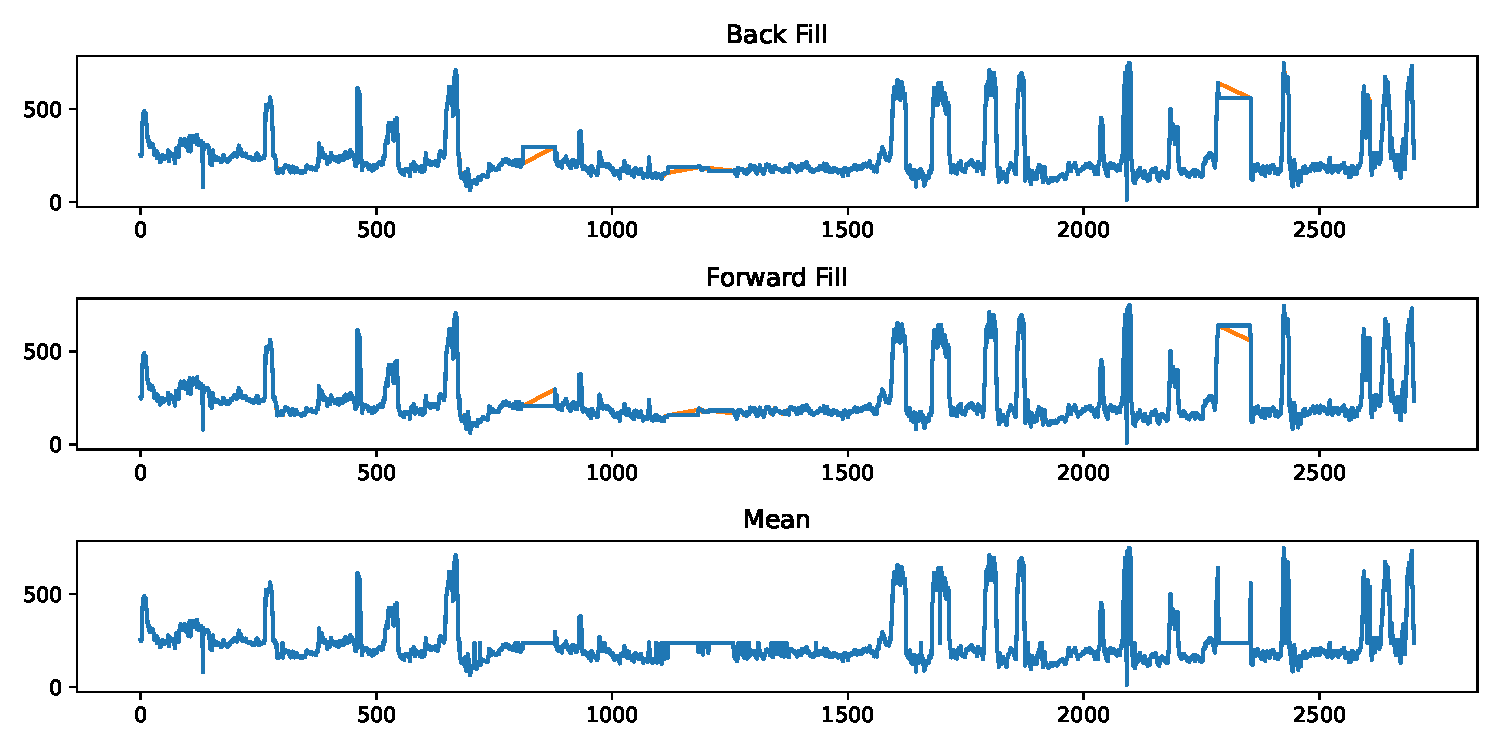
\includegraphics[width = .9\textwidth]{images/fillna_examples.pdf}
\end{center}

\subsection{Categorical}

Next, we might prefer to look at lower resolution data. Cyclists sometimes don't look at the exact output value, but instead focus on staying in some range of values. This lends itself to \link{https://blog.onepeloton.com/power-zone-training/}{power zone training}. 

This means we might use (ordered) \emph{categorical} data. This relies on the pandas \code{Categorical} type. Categories that are numerical intervals can be created with \code{cut()} and \code{qcut()}. You might also work with categories that are simply string names. \code{cut()} takes a sequence of numbers and places it in a numerical category. Below, we set the bins manually based off \code{zone_mins}. Then we can access the created categories with the \code{categories} attribute. There is also the accessor, \code{cat}, which works like the \code{str} string accessor. We use that when creating \code{zone_data}, transforming raw output to zone/categorical data. 

\begin{lstlisting}
ftp = 210
zone_mins = 0, .56*ftp, .76*ftp, .91*ftp, 1.06*ftp, 1.21*ftp, 1.51*ftp, 10**10

# Hacky way to get interval categories
cats = pd.cut([1], bins = zone_mins).categories

zone_data = df.output.astype('category').cat.set_categories(cats1)
zone_data.value_counts()
\end{lstlisting}

The categorical data type has the advantage of better performance and something like \code{value_counts()} behaves slightly different. 

\begin{lstlisting}
# Shows 0 frequencies for high zones
pd.cut([1], zone_mins).value_counts()

# Doesn't show high zones
pd.Categorical([pd.Interval(zone_mins[0],zone_mins[1])]).value_counts()

# Non-Peloton/non-interval example

a1 = pd.Series(['a'])
print(a1.value_counts())

a2 = pd.Series(['a']).astype('category')
a2 = a2.cat.set_categories(['a', 'b'])
print(a2.value_counts())
\end{lstlisting}



\paragraph{Dummy variables} can be added to our dataset next. \code{get_dummies()} works with a array-like data, Series, and DataFrames. You might also call this one-hot encoding. 

\begin{lstlisting}
pd.get_dummies(zone_data)
\end{lstlisting}


